\documentclass[12pt]{article}
\usepackage[spanish]{babel }
\usepackage{graphicx}
\usepackage{float}
\usepackage{hyperref}
\usepackage{times}
%opening
\title{\textbf{\textit{\underline{¿Inundación o sequía?}}}}

\begin{document}
	
\begin{titlepage}
	\centering
	\vspace*{1cm}
	\begin{figure}
		\centering
		
\includegraphics[width=0.3\linewidth]{images/logo}
		\label{fig:logo}
	\end{figure}
	
	\large{\textbf{Universidad de La Habana}\\
	Facultad de Matemática y Computación\\}
	\vspace{3.5cm}
	
	{\rmfamily\selectfont\Huge{¿Inundaciones o sequía?}} 
	\vspace{1.5cm}
	
	\Large
	\vspace{2 cm}
	\normalsize{\textbf{Autores:}\\
		Jennifer de la Caridad Sánchez Santana\\
		Angélica María Martínez Céspedez\\
		Guillermo Ferriol Ravelo\\
		Diego Puentes Fernández\\}
	\vfill
	
	\large
	\today
\end{titlepage}

	
	\begin{center}
		\textbf{\textit{\underline{{\fontsize{60}{24}\selectfont Huracán Ian:}}}}
	\end{center}
	
	
	\begin{figure}[H]
		\centering
		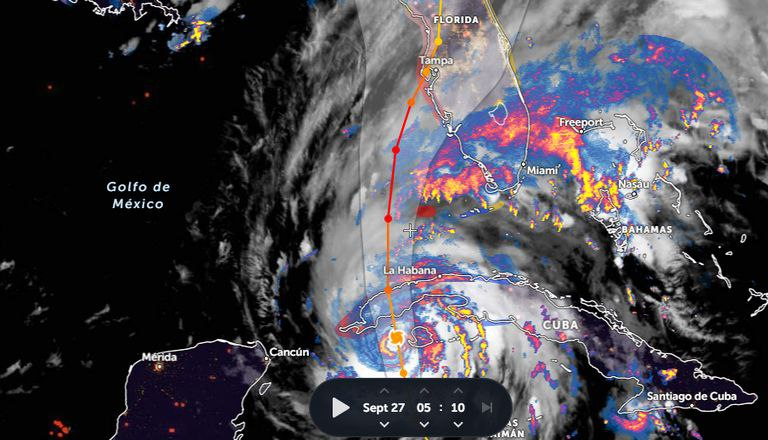
\includegraphics[width=0.7\linewidth]{./Report/images/Ian}
		\label{fig:ian}
	\end{figure}
	
	
	A las 4:40 de la madrugada del día 27 de septiembre del 2022,tocaba tierras cubanas por la provincia de Pinar del Río un intenso huracán de nombre Ian,con vientos máximos sostenidos de 205 km/h,y de categoría 3 de la escala Saffir-Simpson.Durante la mañana de este mismo día,ocurrieron en dicha provincia vientos fuertes en racha y numerosas lluvias,así como inundaciones costeras hacia la costa sur.A las 9:50 am,Ian emergió al sudeste del Golfo de México,quedando aún en algunos pueblos vientos sostenidos de 185 km/h.Ya en la tarde había dejado totalmente la Isla,adentrándose cada vez más en aguas del golfo.En tan solo 7 horas el huracán provoco graves daños en las redes principales y secundarias de suministro de agua,así como en sistema de abastecimiento de varios municipios y derrumbes parciales y totales en varios miles de de viviendas, afectaciones a las coberturas e infraestructura de instituciones públicas,caída de árboles,al suministro de electricidad en el país,inundaciones en zonas bajas así como cuantiosos daños en la agricultura.\cite{webpage1}
	
	
	\begin{figure}[H]
		\centering
		\includegraphics[width=0.6\linewidth]{./Report/images/huracán_Ian}
		\caption{Huracán Ian.}
		\label{fig:huracanian}
	\end{figure}
	
	
	Después de la salida del huracán Ian,las provincias más afectadas por este fenómeno natural fueron Pinar del Río,Artemisa,La Habana y Mayabeque.A excepción de Mayabeque, todas estas provincias experimentaron precipitaciones por encima de la media.Sin embargo,esto no cambia el hecho de que el resto del país estuviera en medio de una extensa sequía.A pesar de las numerosas inundaciones y precipitaciones causadas por el huracán,en el mes de octubre,estas mismas provincias se vieron gravemente afectadas por la sequía.\cite{webpage2}
	
	\begin{figure}[H]
		\centering
		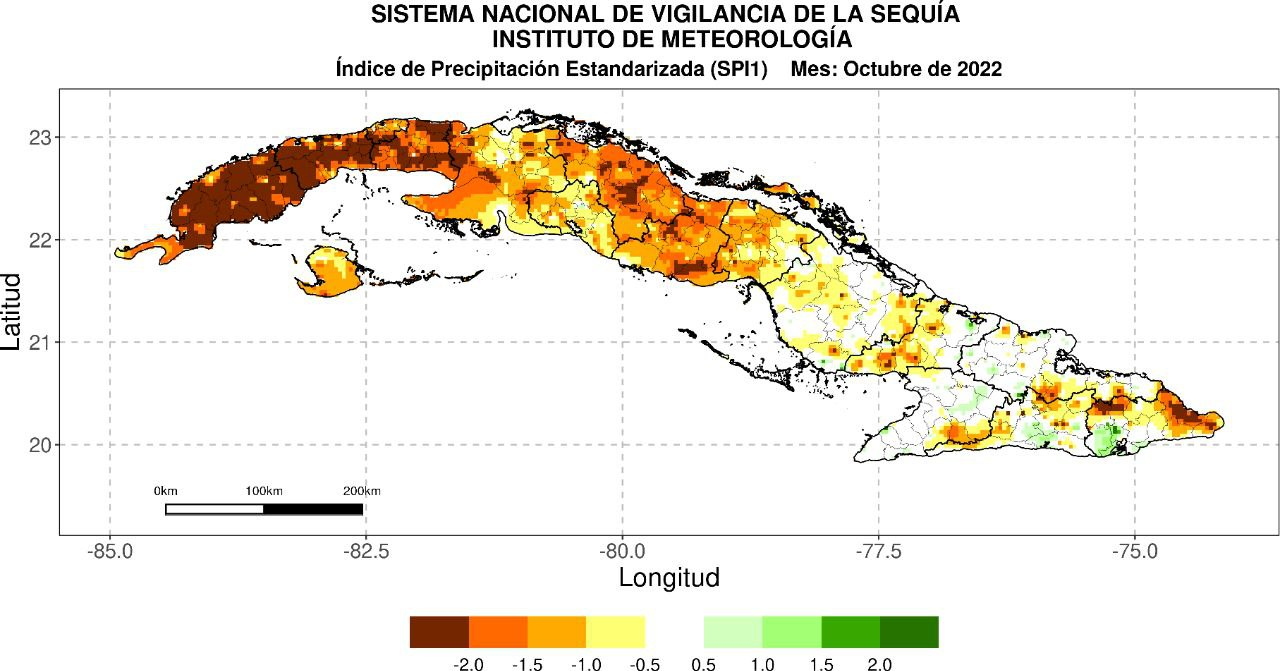
\includegraphics[width=0.8\linewidth]{./Report/images/mapa_octubre_ismet}
		\caption{Mapa de Cuba con las provincias más afectadas en el mes de octubre.}
		\label{fig:mapaoctubreismet}
	\end{figure}
	
	\begin{figure}[H]
		\centering
		\includegraphics[width=0.7\linewidth]{./Report/images/provincias_más_afectadas}
		\caption{Comportamiento de las precipitaciones en las provincias más afectadas.}
		\label{fig:provinciasmasafectadas}
	\end{figure}
	
	
	
	\begin{figure}[H]
		\centering
		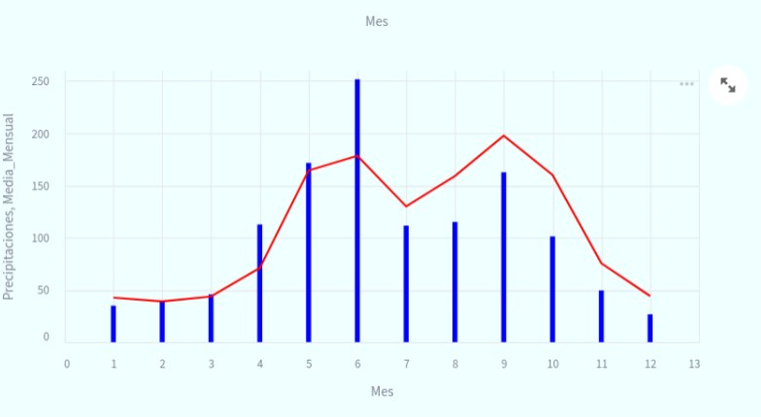
\includegraphics[width=0.8\linewidth]{./Report/images/precipitaciones_2022}
		\caption{Comportamiento de las precipitaciones por mes en 2022.}
		\label{fig:precipitaciones2022}
	\end{figure}
	
	
	\newpage
	Esto nos dirige a la siguiente pregunta:
	
	\textbf{¿Los fénomenos naturales que han ocurrido en Cuba,los cuales generan desde numerosas lluvias hasta inundaciones,aportan suficiente agua como para apasiguar la sequía?}\\
	
	
	Según el sitio web "Periodismo de Barrio",las sequías más extensas de este siglo ocurrieron en un período específico de años,es decir,de \textbf{2003-2005},de \textbf{2009-2010} y de \textbf{2014-2015}.\textbf{¿Qué paso en esos rangos de años?}\cite{webpage3}
	
	\begin{itemize}
		\item\textbf{Período 2003-2005:}
	\end{itemize}
	
	\begin{figure}[H]
		\centering
		\includegraphics[width=0.9\linewidth]{./Report/images/gráfica_ismet}
		\caption{Tabla del ISMET}
		\label{fig:graficaismet}
	\end{figure}
	
	
	Según el Instituto de Metereología de la República de Cuba,en este período se registraron 3 huracanes,uno de categoría "3" y los otros dos de categoría "4",la escala Saffir-Simpson.Estos huracanes ocasionaron inundaciones en algunas provincias como Santiago de Cuba,Matanzas y la Isla de la Juventud.\cite{webpage4}
	
	
	\begin{figure}[H]
		\centering
		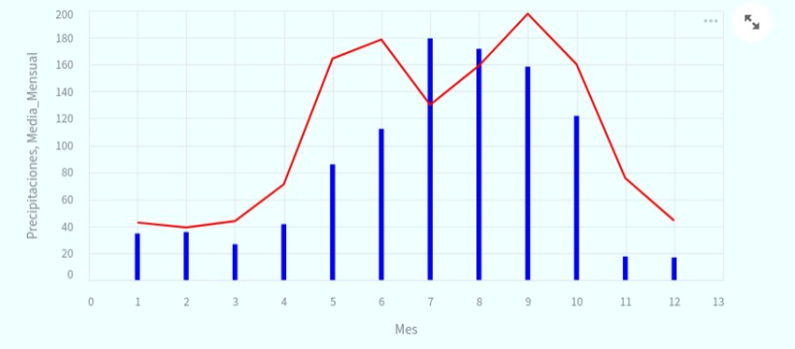
\includegraphics[width=0.7\linewidth]{./Report/images/precipitaciones_2004}
		\caption{Comportamiento de las precipitaciones en 2004.}
		\label{fig:precipitaciones2004}
	\end{figure}
	
	
	\begin{figure}[H]
		\centering
		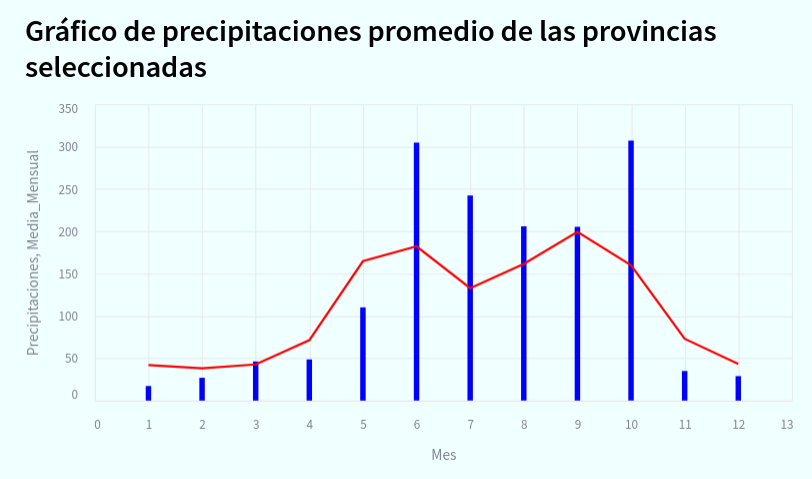
\includegraphics[width=0.7\linewidth]{./Report/images/precipitaciones_2005}
		\caption{Comportamiento de las precipitaciones en 2005.}
		\label{fig:precipitaciones2005}
	\end{figure}
	
	
	Lo interesante es que justo en esos mismos meses,se produjó una de las\textbf{ más grandes sequías registradas en los últimos 50 años.}\cite{webpage5}
	
	
	\begin{figure}[H]
		\centering
		\includegraphics[width=0.8\linewidth]{./Report/images/tabla_peligro_sequía}
		\caption{Tabla de peligro de sequía.}
		\label{fig:tablapeligrosequia}
	\end{figure}
	
	\begin{itemize}
		\item\textbf{Período 2009-2010:}
	\end{itemize}
	
	
	En 2009,Cuba experimentó una temporada ciclónica muy inactiva,con poca actividad de fenómenos naturales.En contraste,en 2010,el país fue afectado por la "Depresión Tropical Paula",que trajo consigo abundantes precipitaciones al centro del país.Estas lluvias fueron positivas en esa región,ya que ayudaron a mitigar los efectos de la sequía,al menos en ese mes y esa área en específico.\cite{webpage6}\cite{webpage7}
	
	\begin{figure}[H]
		\centering
		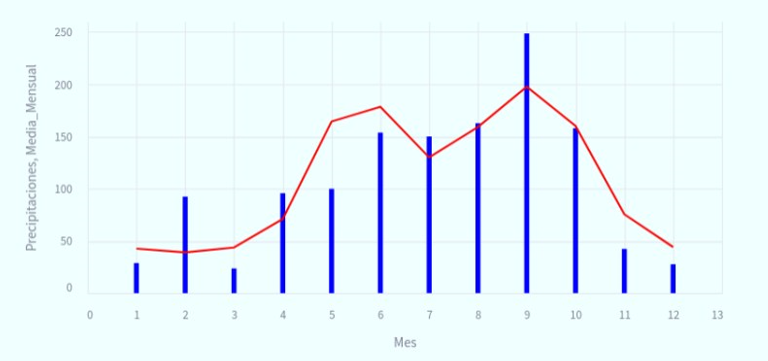
\includegraphics[width=0.6\linewidth]{./Report/images/precipitaciones_2010}
		\caption{Comportamiento de las precipitaciones en el 2010.}
		\label{fig:precipitaciones2010}
	\end{figure}
	
	
	\begin{figure}[H]
		\centering
		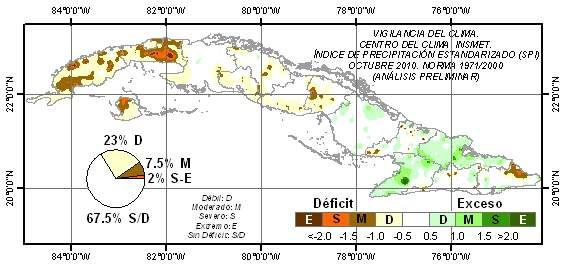
\includegraphics[width=0.7\linewidth]{./Report/images/mapa}
		\caption{Mapa de Cuba de precipitación de octubre del 2010}
		\label{fig:mapa}
	\end{figure}
	
	\begin{itemize}
		\item \textbf{Período 2014-2015:}
	\end{itemize}
	
	
	En 2014,no ocurrieron muchos fenómenos naturales durante la temporada ciclónica,lo que la hizo bastante inactiva.Sin embargo,en 2015,el huracán "Joaquín" no pasó directamente por la Isla,pero afectó varias provincias,desde Ciego de Ávila hasta Guantánamo,provocó fuertes lluvias,tormentas eléctricas,marejadas e inundaciones costeras en los primeros días de octubre.Estas lluvias ayudaron a mitigar los efectos de la sequía en esas zonas y meses específicos.\cite{webpage6}\cite{webpage8}
	
	\begin{figure}[H]
		\centering
		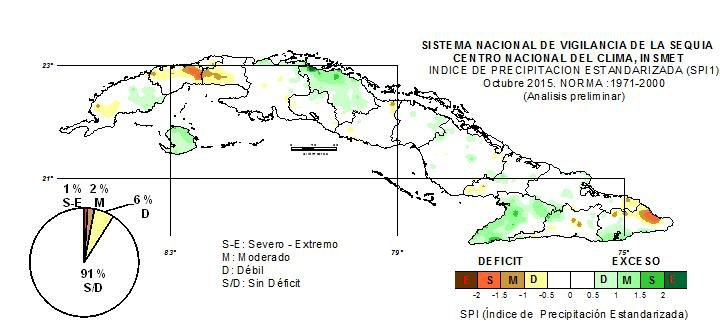
\includegraphics[width=0.7\linewidth]{./Report/images/mapa_octubre_2015}
		\caption{Mapa de Cuba de precipitación de octubre del 2015.}
		\label{fig:mapaoctubre2015}
	\end{figure}
	
	
	
	En conclusión,la interacción entre huracanes e inundaciones con períodos de sequía en Cuba plantea desafíos significativos para la gestión del agua y la adaptación al cambio climático.A pesar de las lluvias intensas asociadas a los huracanes,las provincias afectadas por estos fenómenos continúan experimentando sequías,lo que destaca la complejidad de los impactos climáticos en la disponibilidad de agua.La necesidad de estrategias sostenibles para la gestión de recursos hídricos y la adaptación a la variabilidad climática se vuelve cada vez más urgente.A través del análisis de eventos pasados y la comprensión de sus impactos,se pueden extraer lecciones valiosas para enfrentar futuros desafíos climáticos y garantizar la seguridad hídrica en Cuba. Recuerden que siempre es importante cuidar nuestro planeta,nuestra tierra,y contribuir a este de todas las formas posibles.Ahorra agua!.
	
	
	\begin{figure}[H]
		\centering
		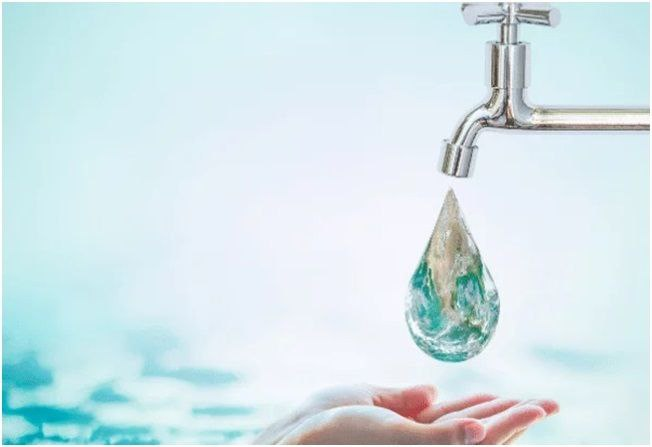
\includegraphics[width=0.4\linewidth]{./Report/images/agua}
		\label{fig:agua}
	\end{figure}
	
	
	\newpage
	\begin{thebibliography}{8}
		\bibitem{webpage1} 
		\url{chttps://www.unicef.org/cuba/huracan-ian-cuba}
		
		\bibitem{webpage2}
		\url{http://www.insmet.cu/asp/genesis.asp?TB0=PLANTILLAS&TB1=sqCLIMA&TB2=/clima/Sequia/SQOCTUBRE2015.HTM&TB3=2015}
		
		\bibitem{webpage3}
		\url{https://periodismodebarrio.org/2023/11/las-sequias-en-cuba-explicadas/amp/}
		
		\bibitem{webpage4}
		\url{https://rcm.insmet.cu/index.php/rcm/article/view/493/768}
		
		\bibitem{webpage5}
		\url{http://rcm.insmet.cu/index.php/rcm/article/download/186/127/0
			http://rcm.insmet.cu/index.php/rcm/article/download/186/127/0}
		
		\bibitem{webpage6}
		\url{http://www.insmet.cu/asp/genesis.asp?TB0=PLANTILLAS&TB1=TEMPORADA&TB2=/Temporadas/temporada2020.html}
		
		\bibitem{webpage7}
		\url{http://www.cubadebate.cu/temas/medio-ambiente-temas/2010/11/30/termina-hoy-la-activa-temporada-ciclonica-del-2010/amp/}
		
		\bibitem{webpage8}
		\url{http://www.cubadebate.cu/noticias/2015/10/01/nota-informativa-no-1-del-estado-mayor-nacional-de-la-defensa-civil-sobre-el-huracan-joaquin/amp/}
		
	\end{thebibliography}
	
	
\end{document}